\documentclass[entwurf.tex]{subfiles}

\begin{document}

\chapter{Sequenzdiagramme}
	\section{Verbindung zwischen Client und Server herstellen}
	\label{Sequence:TerminalConnect}
		In dem folgenden Diagramm sieht man den Ablauf des Verbindens eines Endgeräts mit dem Server. Auf die Ausführung des Verbindens folgt in der Regel ''\nameref{Sequence:LiveDataNewConfig}''
		
		In diesem Fall handelt es sich beim Terminal um das Endgerät, auf dem über einen Browser die VINJAB-Seite aufgerufen wird. Der Befehl openWebpage() soll das Aufrufen der Website darstellen. Es handelt sich sozusagen um eine Anfrage über HTTP nach den genutzten Dateien und Programmteilen. Bei der Referenz für die WebRTC-Connection wird ''\nameref{Sequence:WebRTCConnect}'' ausgeführt.
		
		\begin{figure}[H]
 			\makebox[\textwidth][c]{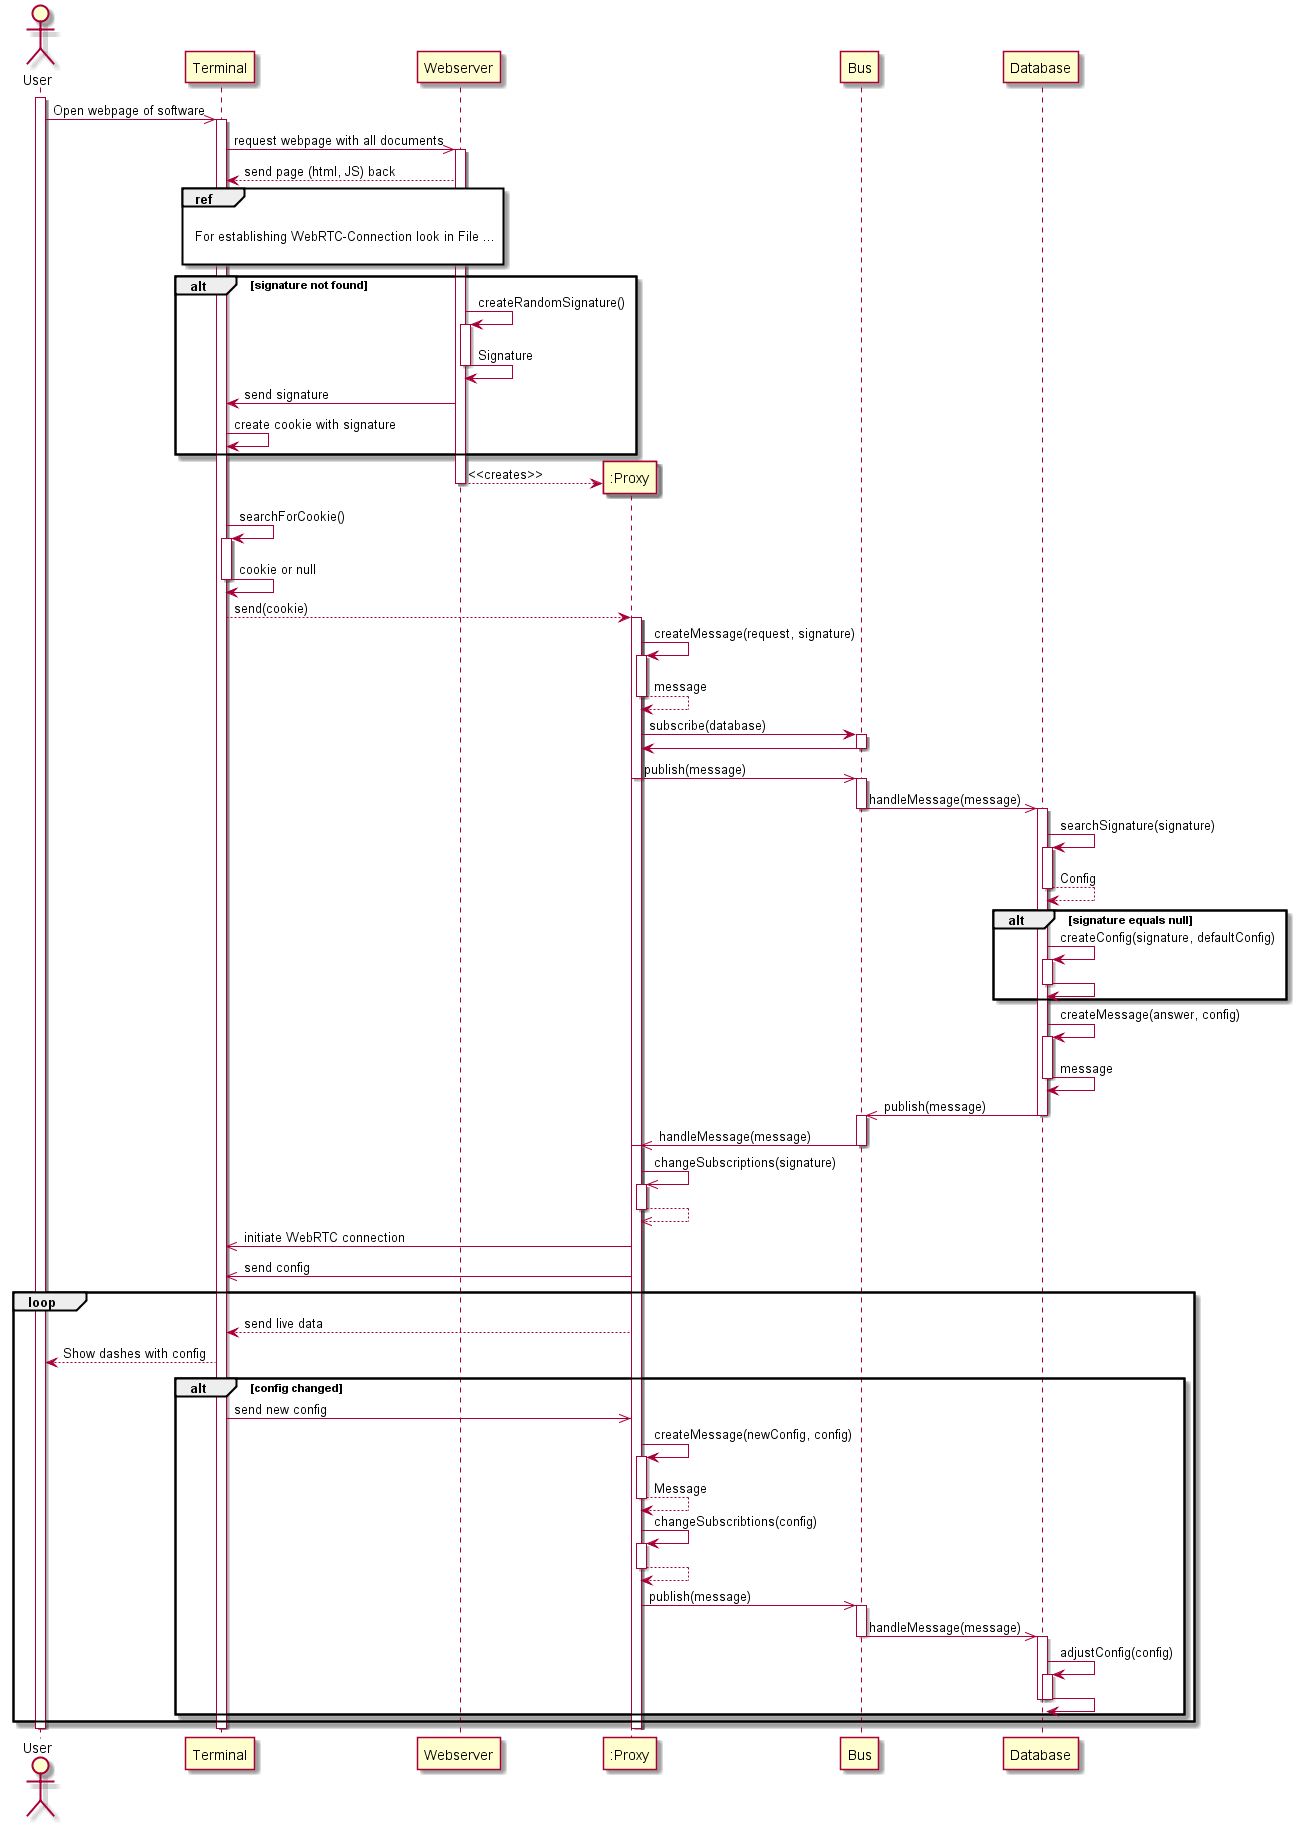
\includegraphics[width=0.9\paperwidth]{diagrams/Connect.png}}
  			\caption{Herstellen einer Verbindung zwischen Client und Server}
  		\end{figure}
  		
  	\section{WebRTC-Verbindung herstellen}
  	\label{Sequence:WebRTCConnect}
		In dem folgenden Diagramm wird dargestellt, wie eine WebRTC-Verbindung zwischen dem Endgerät und dem Webserver hergestellt wird. Bei unserem Projekt initiiert der Client die Verbindung.
		
		\begin{figure}[H]
			\begin{center}
	 			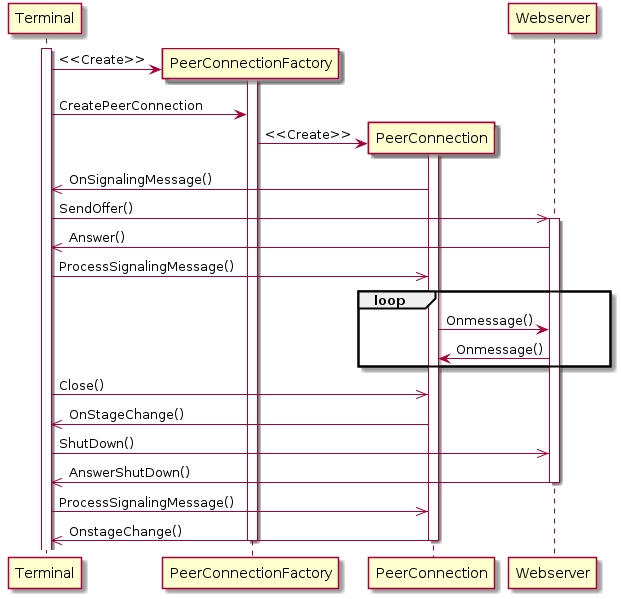
\includegraphics[width=\textwidth]{diagrams/DataTransferSequenz.png}
  				\caption{Herstellen einer WebRTC-Verbindung}
  			\end{center}
  		\end{figure}
  		
  	\newpage
  	\section{Livedaten und Konfiguration}
  	\label{Sequence:LiveDataNewConfig}
  		Nach hergestellter Verbindung befindet sich das System in einer Schleife, in der eigentlich nur noch Live-Daten vom Server zum Client geschickt werden. Nur wenn der Nutzer die Anzeigeeinstellungen ändert, wird diese Schleife für kurze Zeit unterbrochen, um die neue Konfiguration an den Server zu übermitteln, damit von diesem keine nicht benötigten Daten mehr versendet werden und die Konfiguration permanent gespeichert werden kann.
  		\begin{figure}[H]
  			\begin{center}
 				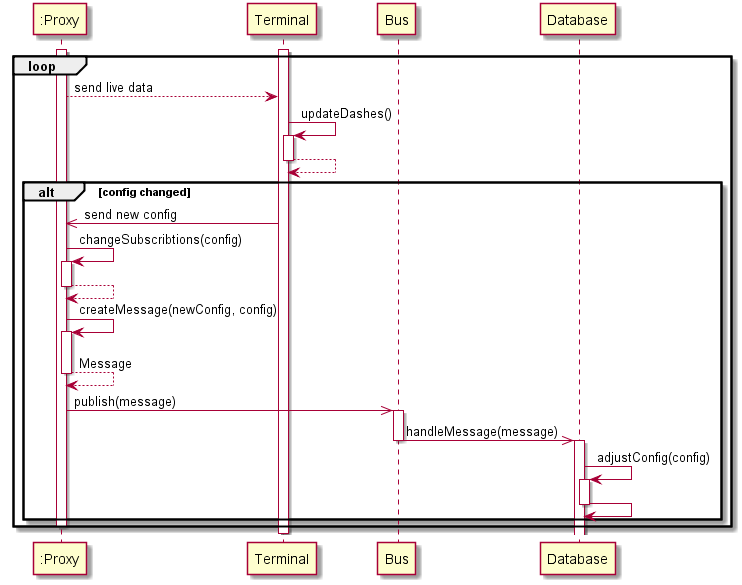
\includegraphics[width=\textwidth]{diagrams/ChangeDashConfig.png}
  				\caption{Livedatenübertragung und Konfigurationsänderung}
  			\end{center}
  		\end{figure}
  		
  	\section{Statistik übertragen}
  		\subsection{Aggregierte Funktionen anfordern}

      Der User fordert ein Dash zur Anzeige an, welches bisher noch nicht angezeigt wurde. Über die Peer Connection von WebRTC wird eine \elqq RequestMessage\erqq{} an den Server geschickt. Auf Serverseiter wird vom entsprechenden TerminalProxy eine RequestMessage für den entsprechenden Wert auf den Bus gelegt. Der Erzeuger verabeitet die Nachricht und veröffentlicht ab sofort die erzeugten Werte auf dem Bus. Handelt es sich beim Erzeuger um einen virtuellen Sensor, muss dieser noch einen Request an die Datenbank senden, sofern ein Diagramm oder Durchschnittswert gefragt ist. Die Datenbank hat eine Fassade, die ein Bus Device ist.

  		\begin{figure}[H]
 			\makebox[\textwidth][c]{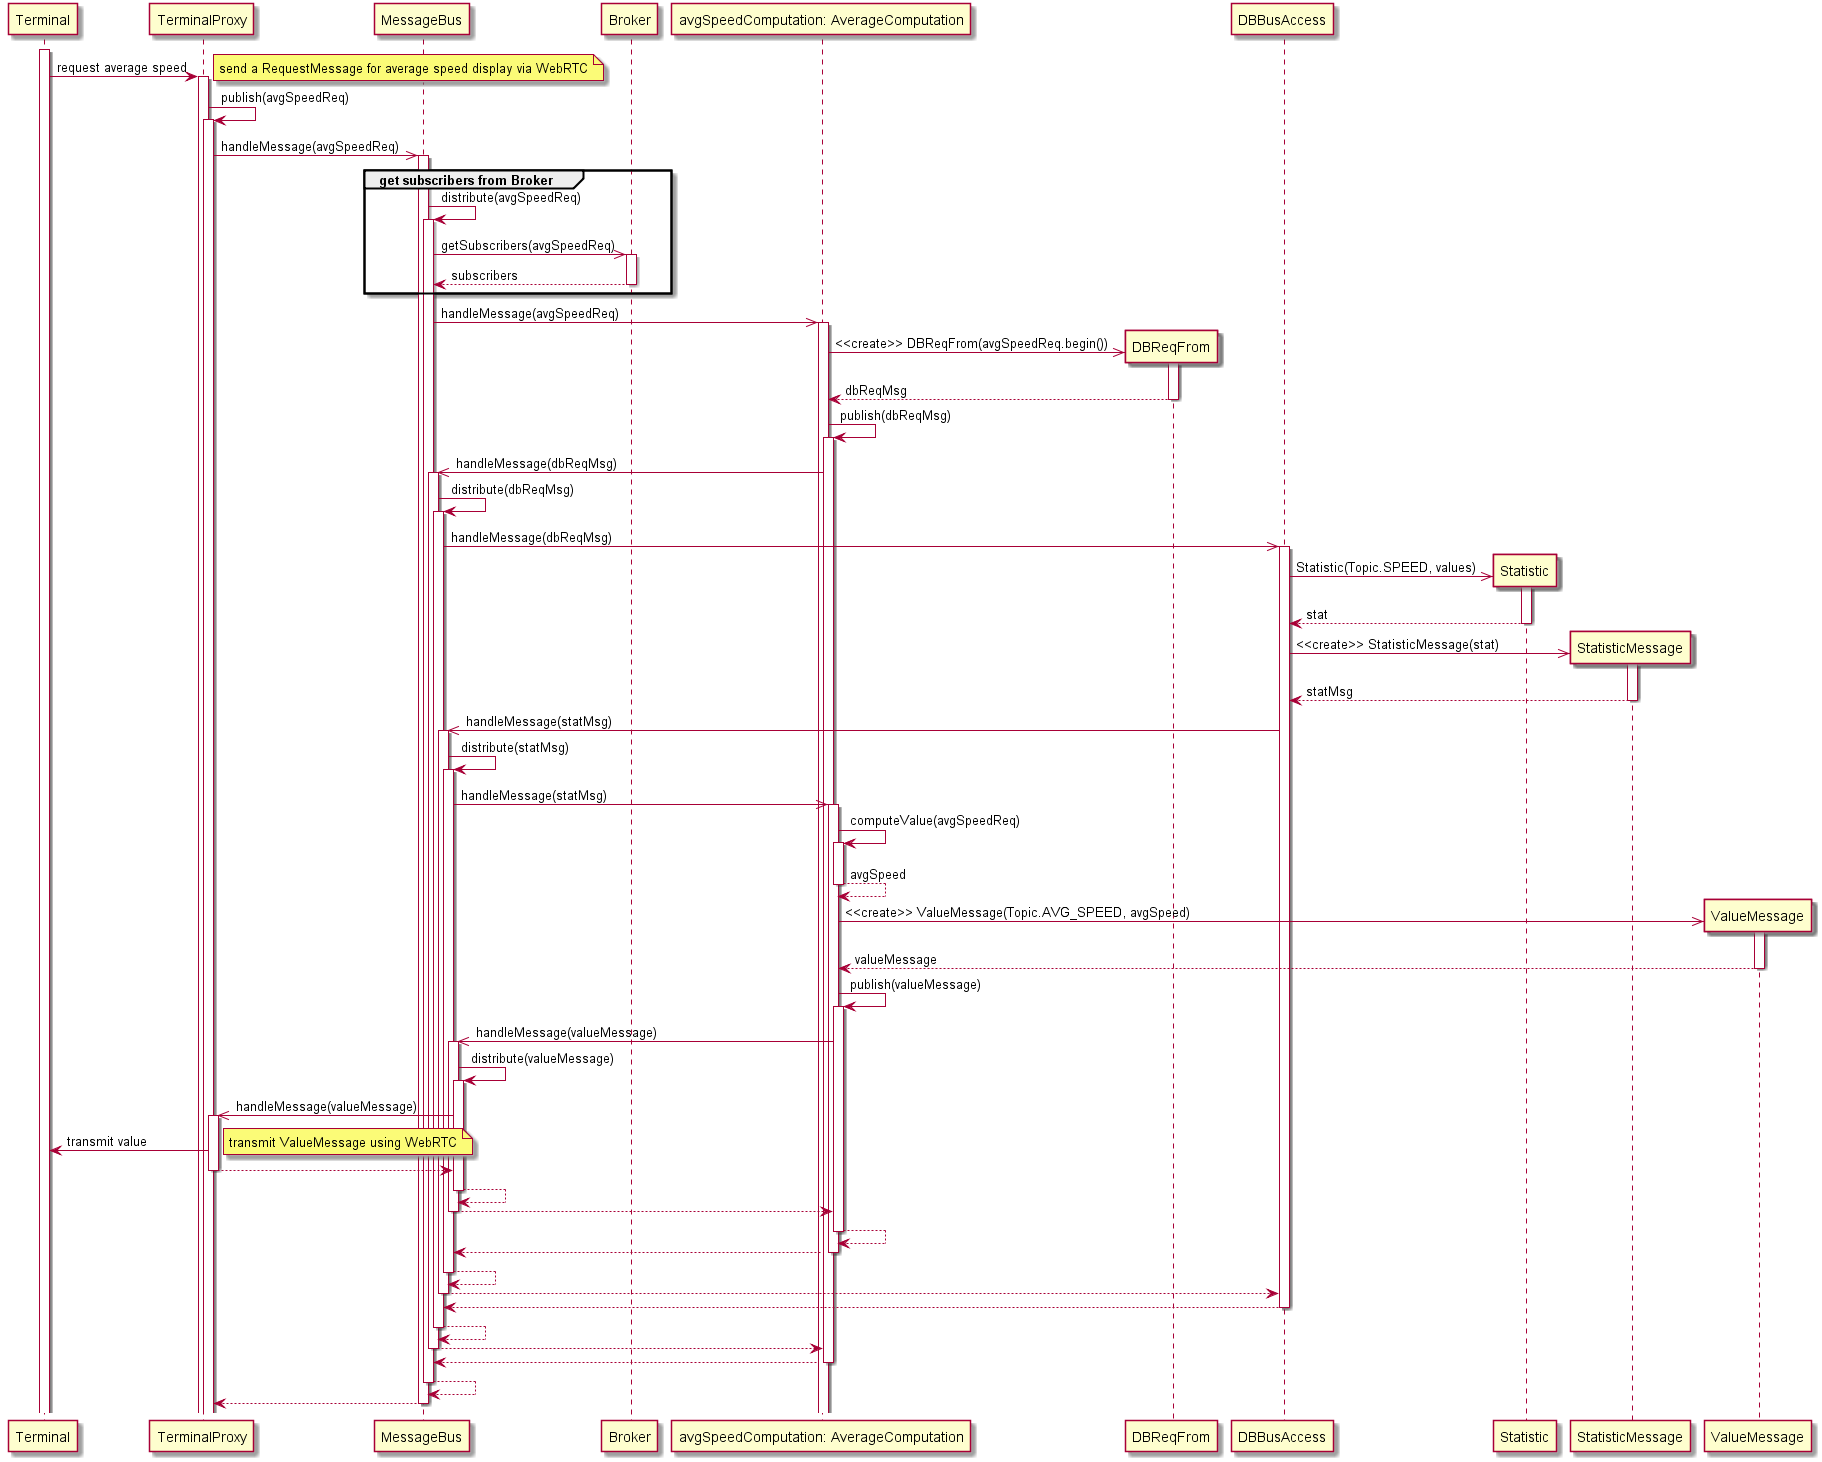
\includegraphics[width=0.9\paperwidth]{diagrams/StatsDBSeq.png}}
  			\caption{Verschiedene Dash-Anzeigeelemente.}
  		\end{figure}
  		
  	
\end{document}